\documentclass[8pt]{beamer}


\usepackage{beamerthemeMunichHH}
\usepackage{amsmath,amssymb,amsthm}
\usepackage{verbatim,fancyvrb}

\usepackage{graphicx}
\usepackage{wrapfig}
\usepackage{caption}
\usepackage{subcaption}
\usepackage[utf8]{inputenc}
\usepackage[german]{babel}
\usepackage[babel, german=quotes]{csquotes}
\usepackage{hyperref}
\usepackage[style=alphabetic]{biblatex}

\addbibresource{bibliography.bib}

% ------------------------------------------------------------------------
% font management
% ------------------------------------------------------------------------

\usepackage{euler}
\renewcommand{\familydefault}{\sfdefault}
\renewcommand{\rmdefault}{\familydefault}

\usepackage{mathrsfs} % for mathscr font

% ------------------------------------------------------------------------
% References Logistics
% ------------------------------------------------------------------------

\usepackage{lmodern}    
\usepackage[labelformat=empty,font=scriptsize,skip=0pt,justification=justified,singlelinecheck=false]{caption}

%remove the icon
\setbeamertemplate{bibliography item}{}

%remove line breaks
\setbeamertemplate{bibliography entry title}{}
\setbeamertemplate{bibliography entry location}{}
\setbeamertemplate{bibliography entry note}{}

%\usepackage[backend=bibtex,style=alphabetic,firstinits=true,sorting=none]{biblatex}

% google(beamer printbibliography icon does not appear)
% https://tex.stackexchange.com/questions/124256/how-do-i-get-numbered-entries-in-a-beamer-bibliography
\setbeamertemplate{bibliography item}{\insertbiblabel}

\bibliography{mainRefs}

\makeatletter
\def\blx@maxline{77}
\makeatother

% ------------------------------------------------------------------------
\title{Support Vector Machines mit Kerneln}
\author{Tim Schlottmann, Hendrik Sieck, Jonas Krug}
\date{26.01.2018}
% ------------------------------------------------------------------------
 
\setbeamercolor{black30}{fg=black!30}

%--------------------------------------------------------------------------
% macros
% ------------------------------------------------------------------------
\def\cA{{\mathcal A}}
\def\cB{{\mathcal B}}
\def\cE{{\mathcal E}}
\def\cG{{\mathcal G}}
\def\cC{{\mathcal C}}
\def\cM{{\mathcal M}}
\def\cN{{\mathcal N}}
\def\cH{{\mathcal H}}
\def\cU{{\mathcal U}}
\def\cX{{\mathcal X}}
\def\cY{{\mathcal Y}}
\def\cK{{\mathcal K}}
\def\sD{{\mathsf D}}
\def\fJ{{\mathfrak J}}
\def\bU{{\mathbb U}}
\def\bV{{\mathbb V}}
\def\bR{{\mathbb R}}
\def\bT{{\mathbb T}}
\def\scA{{\mathscr A}}
\def\scB{{\mathscr B}}
\def\scC{{\mathscr C}}
\def\scE{{\mathscr E}}
\def\scH{{\mathscr H}}
\def\scX{{\mathscr X}}

% ===================================

\newcommand{\pd}[2]{\frac{\partial#1}{\partial#2}}      %% partial deriv
\newcommand{\pdd}[2]{\frac{\partial^2#1}{\partial#2^2}} %% partial deriv

% ===================================

\def\<#1,#2>{\langle#1,#2\rangle} %% inner product (Dirac not'n)

\newtheorem{thm}{Theorem}[section]
\newtheorem{prop}{Proposition}[section]
\newtheorem{defi}{Definition}[section]
\newtheorem{lemm}{Lemma}[section]
\newtheorem{exmp}{Example}[section]
\newtheorem{conj}{Conjecture}[section]
\newtheorem{seti}{Setting}[section]
\newtheorem{obje}{Objectives}[section]
\newtheorem{frmk}{}[section]


%--------------------------------------------------------------------------
% Beamer logistics 
% ------------------------------------------------------------------------

\setbeamertemplate{navigation symbols}{}
\setbeamertemplate{footline}[page number]{}
\setbeamercovered{transparent}
% the following is automatically updated after two compilations
% \renewcommand{\inserttotalframenumber}{12} 

% =============================================================
% prepare the footnote that will appear in the whole document 
\setbeamerfont{pa}{size=\footnotesize}
\setbeamerfont{pb}{size=\tiny}
\setbeamercolor{bblack40}{bg=black!40}
\setbeamercolor{black40}{fg=black!50}


\setbeamertemplate{footline}
{
\hskip7mm \begin{beamercolorbox}[wd=120mm]{white}
{\usebeamerfont{pb}\usebeamercolor[fg]{black}{
\hskip 110mm  \insertpagenumber\,/\,\inserttotalframenumber}}
\begin{beamercolorbox}[sep=1.5pt,wd=115mm]{white}    \end{beamercolorbox}\par
\end{beamercolorbox}
}

% =============================================================
% prepare logos for initial page 
\pgfdeclareimage[height=1.0cm]{uniHHLogo}{tuhhLogo}
\pgfdeclareimage[height=1.0cm]{depmatLogo}{Mathe-Logo}
\usepackage[absolute,overlay]{textpos}
\setlength{\TPHorizModule}{1mm}
\setlength{\TPVertModule}{1mm}

\newcommand{\MyLogoA}{%
\begin{textblock}{14}(2.0,0.9)
  \pgfuseimage{uniHHLogo}
\end{textblock}
}

\newcommand{\MyLogoB}{%
\begin{textblock}{14}(90.0,0.9)
  \pgfuseimage{depmatLogo}
\end{textblock}
}



\begin{document}

  \frame{\titlepage\MyLogoA\MyLogoB}

  %%%%%%%%%%%%%%%%%%%%%%%%%%%%%%%%%%%%%%%%%%%%%%%%%%%%%%%%%%%%%%%%%%%%%%%%%%%%%%%%
% Folie 1: Motivation
%%%%%%%%%%%%%%%%%%%%%%%%%%%%%%%%%%%%%%%%%%%%%%%%%%%%%%%%%%%%%%%%%%%%%%%%%%%%%%%%
\begin{frame}
    \frametitle{Motivation}

    \begin{figure}[h]
        \centering{
            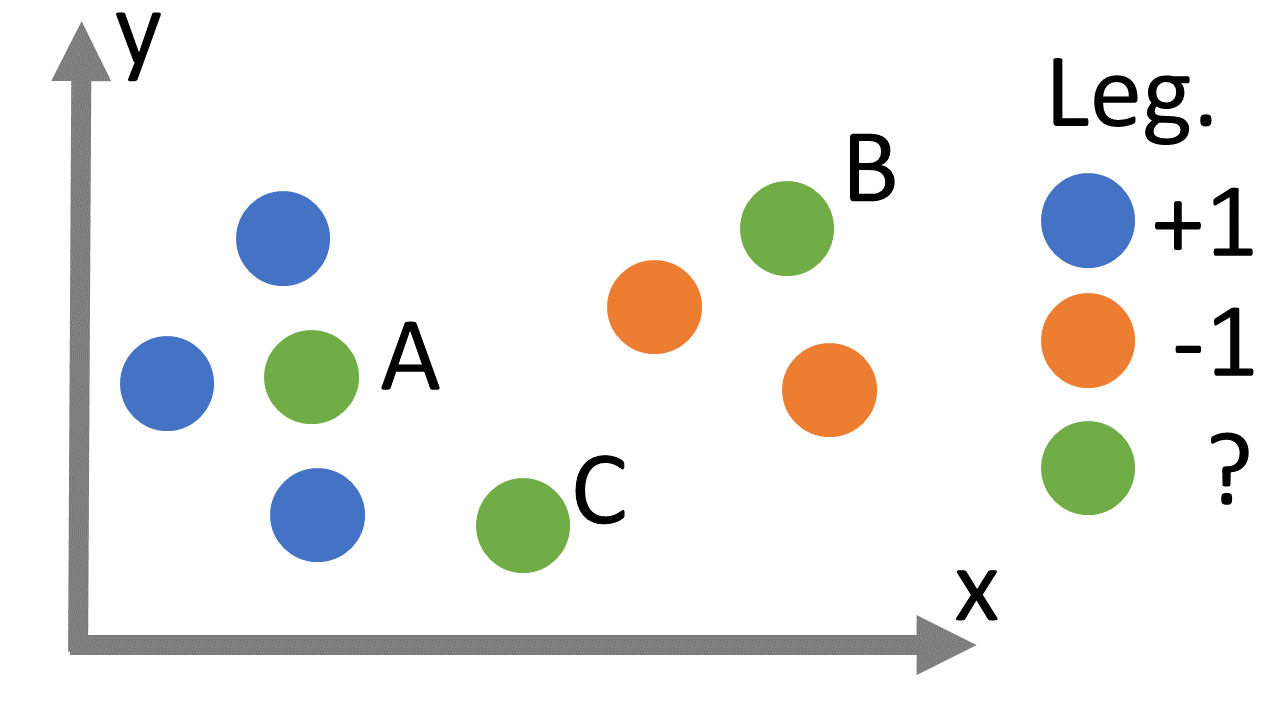
\includegraphics[width=0.5\linewidth]{PowerPoint/Folie1.png}
            % \caption{Beispiel eines Training-Sets mit zu klassifizierenden Punkten}
            \label{motivation:fig_1}
        }
    \end{figure}

    \vspace{3mm}

    \begin{itemize}
        \item Klassifizierung von Objekten
        \item Schnell und effizient
        \item Möglichst genau
    \end{itemize}
\end{frame}

%%%%%%%%%%%%%%%%%%%%%%%%%%%%%%%%%%%%%%%%%%%%%%%%%%%%%%%%%%%%%%%%%%%%%%%%%%%%%%%%
%Folie 2: Themenvorstellung
%%%%%%%%%%%%%%%%%%%%%%%%%%%%%%%%%%%%%%%%%%%%%%%%%%%%%%%%%%%%%%%%%%%%%%%%%%%%%%%%
\begin{frame}
    \frametitle{Themenvorstellung}

    \begin{figure}[h]
        \centering{
            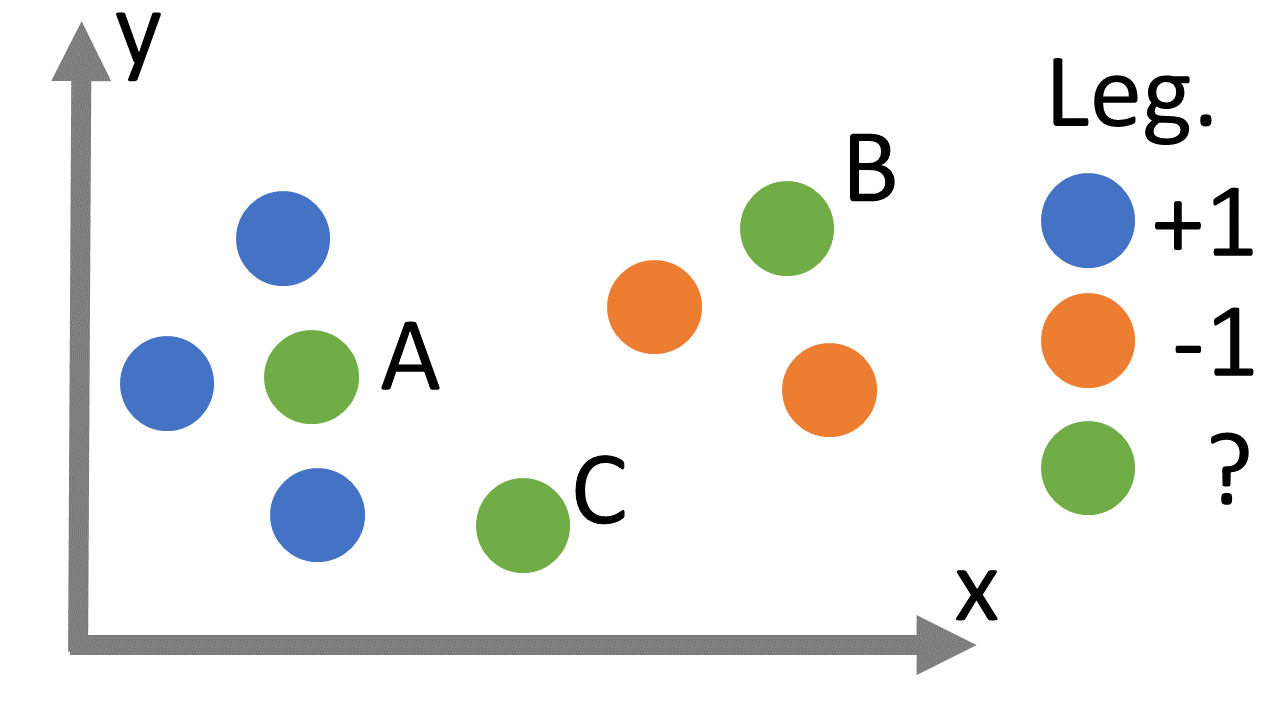
\includegraphics[width=0.5\linewidth]{PowerPoint/Folie1.png}
            % \caption{Beispiel eines Training-Sets mit zu klassifizierenden Punkten}
            \label{themenvorstellung:fig_1}
        }
    \end{figure}

    \vspace{3mm}

    \begin{itemize}
        \item Support Vector Machines (deutsch: Stützvektor Maschine)
        \item Binärer Klassifierierer
    \end{itemize}
\end{frame}

%%%%%%%%%%%%%%%%%%%%%%%%%%%%%%%%%%%%%%%%%%%%%%%%%%%%%%%%%%%%%%%%%%%%%%%%%%%%%%%%
%Folie 3: Lineare Klassifizierung
%%%%%%%%%%%%%%%%%%%%%%%%%%%%%%%%%%%%%%%%%%%%%%%%%%%%%%%%%%%%%%%%%%%%%%%%%%%%%%%%
\begin{frame}
    \frametitle{Lineare Klassifizierung}

    \only<1>{
        \begin{figure}[h]
            \centering{
                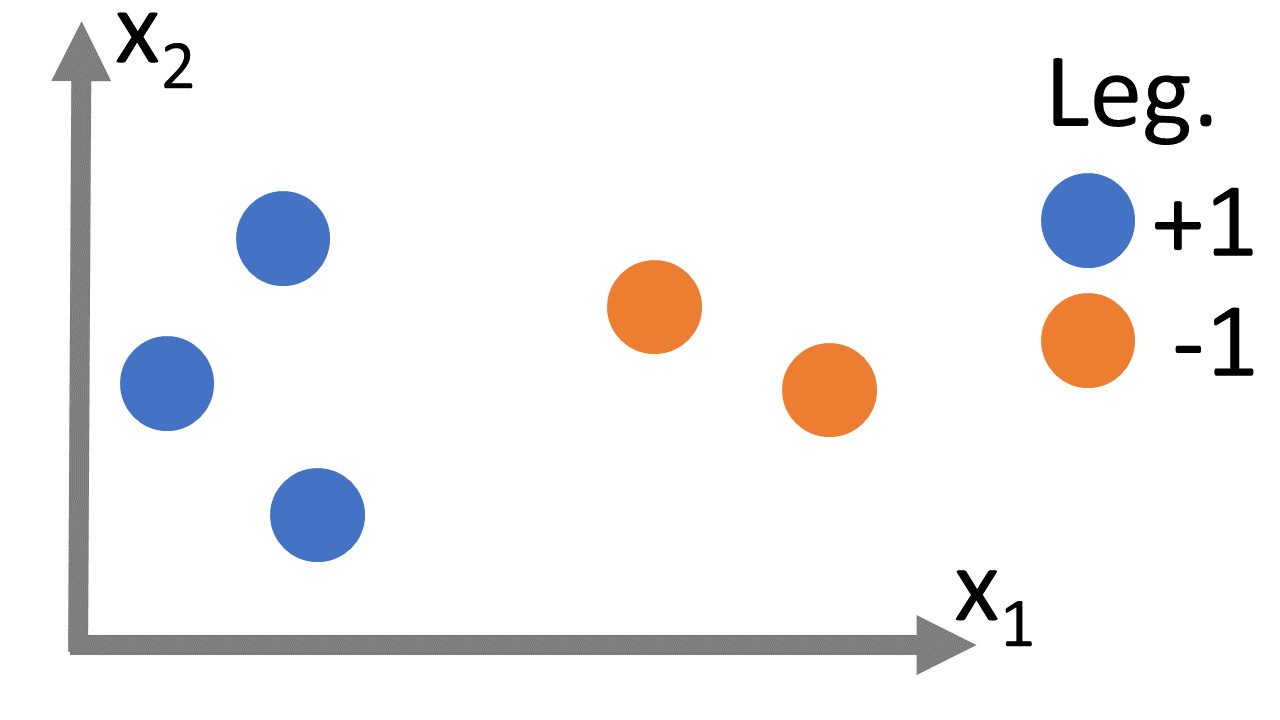
\includegraphics[width=0.5\textwidth]{PowerPoint/Folie2.png}
                % \caption{Beispiel eines Training-Sets}
                \label{lin_klassif:fig_1}
            }
        \end{figure}
    }\only<2>{
        \begin{figure}[h]
            \centering{
                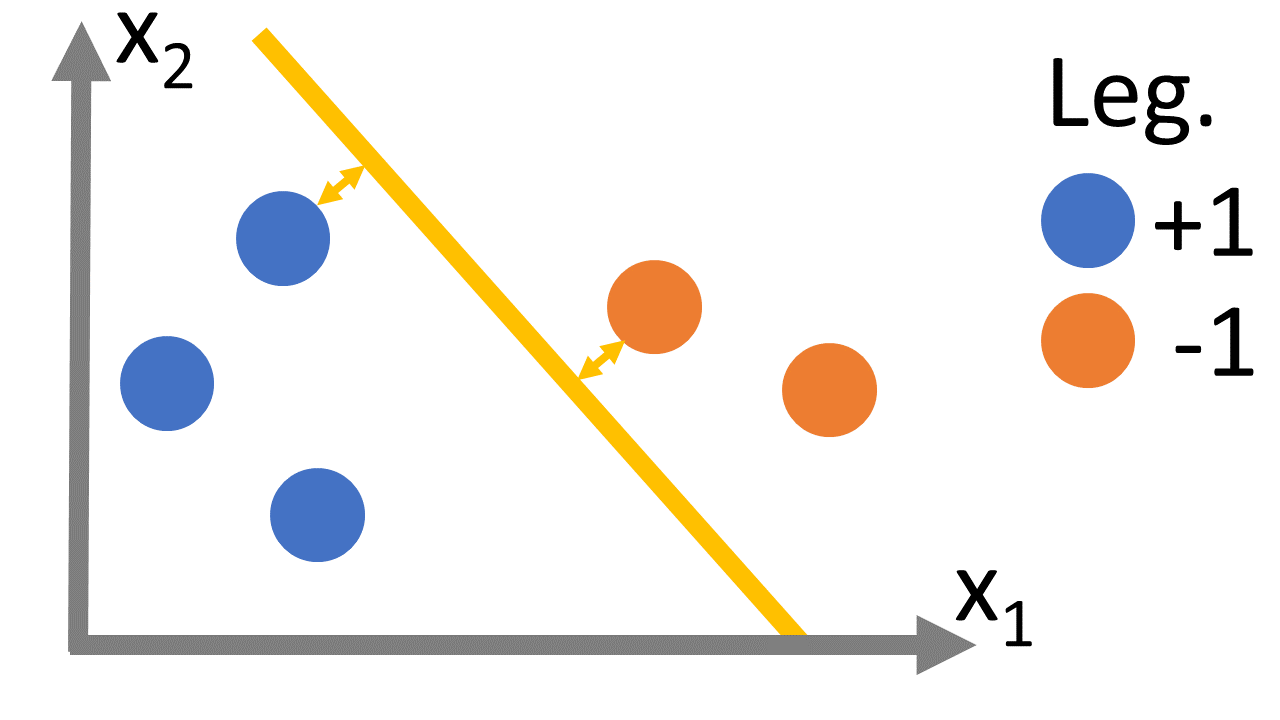
\includegraphics[width=0.5\textwidth]{PowerPoint/Folie3.png}
                % \caption{Beispiel eines Training-Sets}
                \label{definitionen:fig_2}
            }
        \end{figure}
    }\only<3>{
        \begin{figure}[h]
            \centering{
                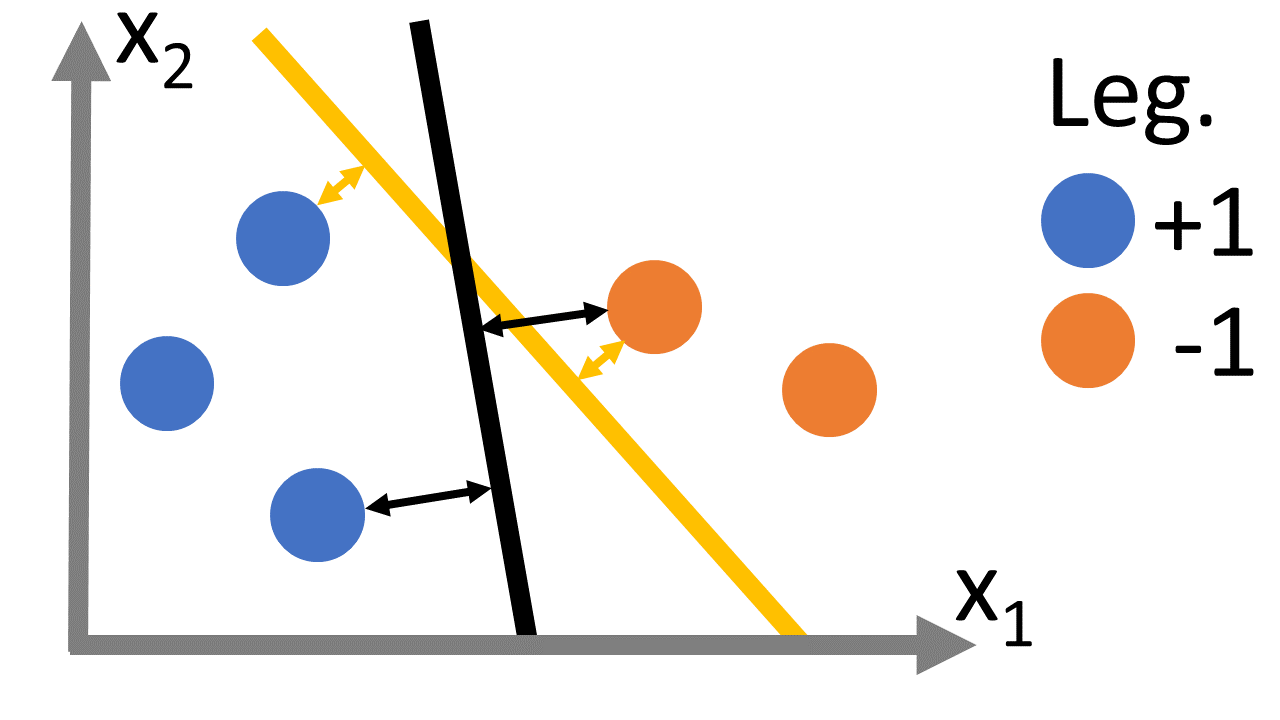
\includegraphics[width=0.5\textwidth]{PowerPoint/Folie4.png}
                % \caption{Beispiel eines Training-Sets}
                \label{definitionen:fig_3}
            }
        \end{figure}
    }\only<4>{
        \begin{figure}[h]
            \centering{
                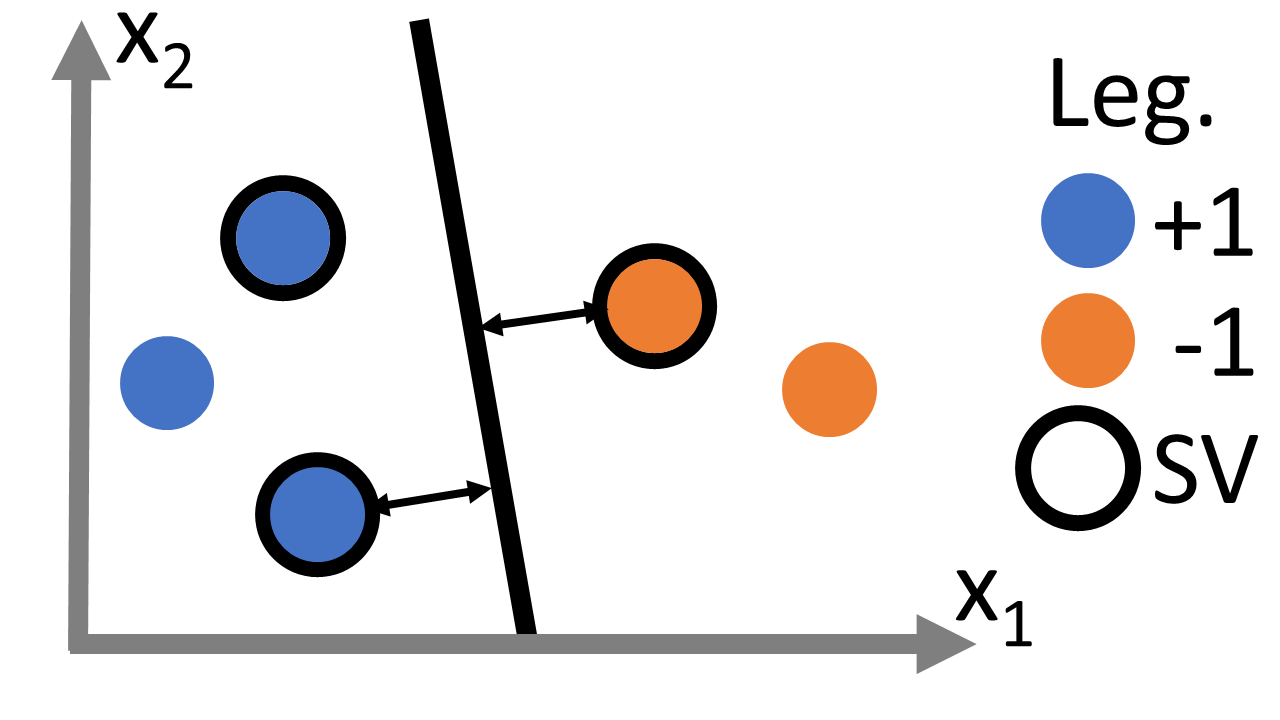
\includegraphics[width=0.5\textwidth]{PowerPoint/Folie5.png}
                % \caption{Beispiel eines Training-Sets}
                \label{definitionen:fig_4}
            }
        \end{figure}
    }

    \only<1>{
        \vspace{3mm}
        
        \begin{itemize}
            \item Wie trenne ich die beiden Klassen voneinander?
        \end{itemize}
    }

    % \only<2->{
    %     \vspace{3mm}

    %     \begin{itemize}
    %         \item Hyperebene: $ \boldsymbol{w} \cdot \boldsymbol{x} + b = 0 $
    %     \end{itemize}
    % }

    \only<2>{
        \vspace{2mm}

        \begin{itemize}
            \item Wie lege ich die Hyperebene am besten?
        \end{itemize}
    }

    \only<3-4>{
        \vspace{2mm}

        \begin{itemize}
            \item Anderer Name von Support Vector Machines: Large Margin Classifier
        \end{itemize}
    }
\end{frame}

%%%%%%%%%%%%%%%%%%%%%%%%%%%%%%%%%%%%%%%%%%%%%%%%%%%%%%%%%%%%%%%%%%%%%%%%%%%%%%%%
%Folie 4: Definitionen
%%%%%%%%%%%%%%%%%%%%%%%%%%%%%%%%%%%%%%%%%%%%%%%%%%%%%%%%%%%%%%%%%%%%%%%%%%%%%%%%
\begin{frame}
    \frametitle{Definitionen}

    \begin{figure}[h]
        \begin{minipage}{0.4\textwidth} 
            \begin{figure}[h]
                \centering{
                    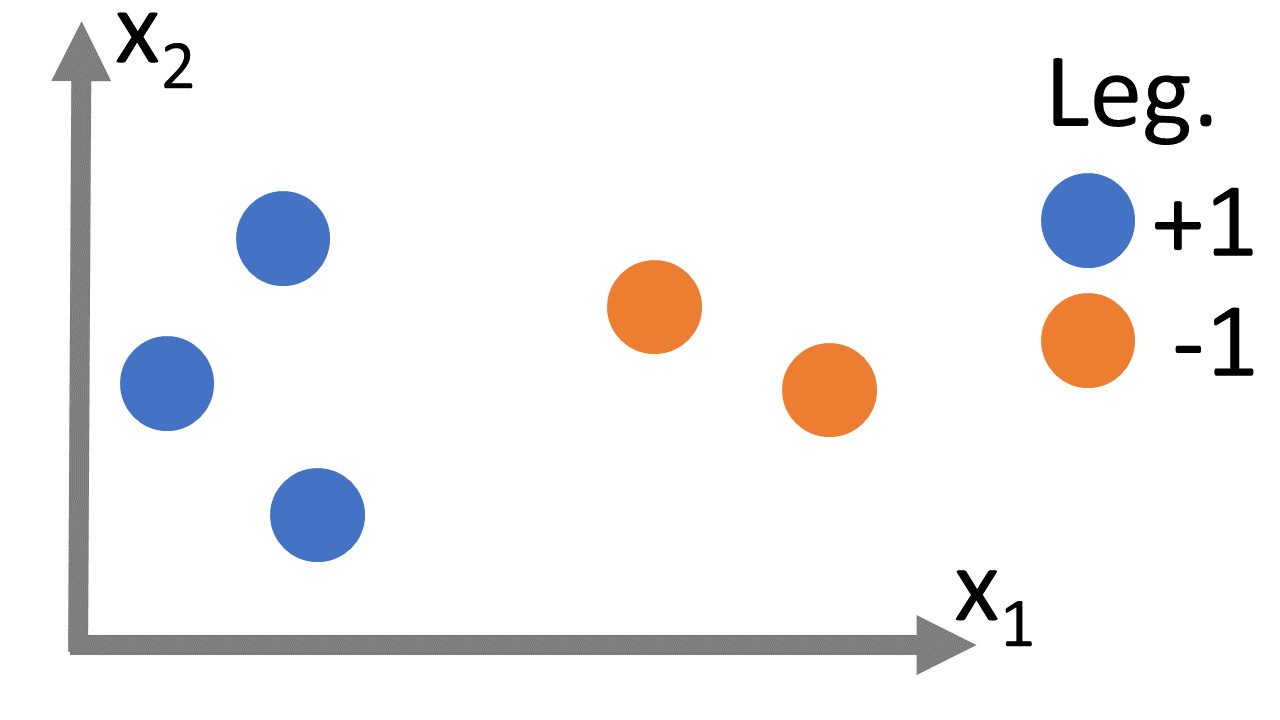
\includegraphics[width=\textwidth]{PowerPoint/Folie2.png}
                    % \caption{Beispiel eines Training-Sets}
                    \label{definitionen:fig_1}
                }
            \end{figure}
        \end{minipage}
        \hfill
        \begin{minipage}{0.4\textwidth}
            \begin{itemize}
                \item<2-> $m = 5$
                \item<2-> Trainingsset:
                    \begin{align*}
                        S &\in (\boldsymbol{x} \times \boldsymbol{y})^m \\
                        &=  \left( \begin{matrix}
                            1 & 0.5 & +1 \\
                            3.5 & 1 & -1 \\
                            & \vdots & \\
                        \end{matrix} \right) \\
                    \end{align*}
            \end{itemize} 
        \end{minipage}
    \end{figure}
    
    \begin{itemize}
        \item Anzahl an Trainingspunkten $ m \in \mathbb{R} $
        \item Input $ \boldsymbol{x} \in \mathbb{R}^N $
        \item Output $ \boldsymbol{y} \in \{ -1, +1 \} $
        \item Trainingsset $S \in (\mathbb{R}^N \times \{ -1, +1 \})^m $
        \item Trainingsset $S \in (\boldsymbol{x} \times \boldsymbol{y})^m $
    \end{itemize}

    \vspace{2mm}

    \begin{itemize}
        \item Hypothese
            \begin{align*}
                h: \boldsymbol{x} &\to \boldsymbol{y} \\
                \boldsymbol{x}_i &\mapsto \{ +1, -1 \} \\
            \end{align*}
    \end{itemize}
\end{frame}

%%%%%%%%%%%%%%%%%%%%%%%%%%%%%%%%%%%%%%%%%%%%%%%%%%%%%%%%%%%%%%%%%%%%%%%%%%%%%%%%
%Folie 5: Large Margin Classifier
%%%%%%%%%%%%%%%%%%%%%%%%%%%%%%%%%%%%%%%%%%%%%%%%%%%%%%%%%%%%%%%%%%%%%%%%%%%%%%%%
\begin{frame}
    \frametitle{Large Margin Classifier}

    \begin{figure}[h]
        \centering{
            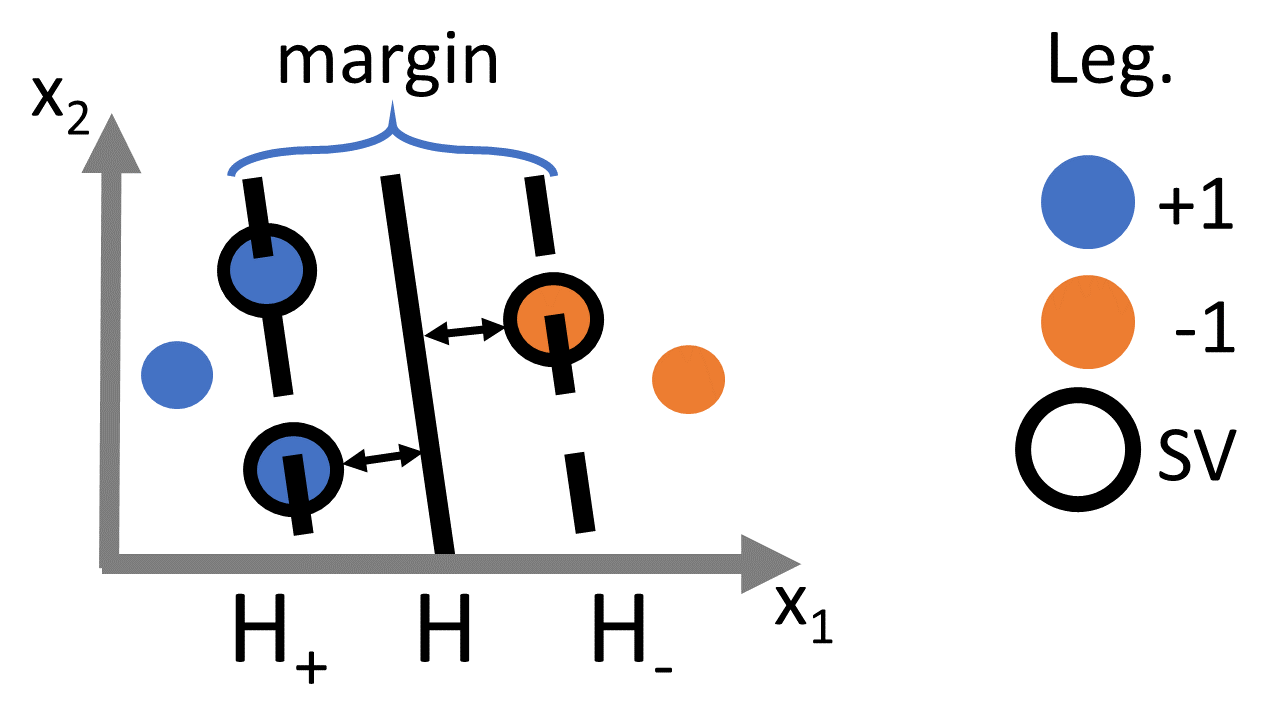
\includegraphics[width=0.5\textwidth]{PowerPoint/Folie7.png}
            % \caption{Beispiel eines Training-Sets}
            \label{large_marg_class:fig_1}
        }
    \end{figure}

    \vspace{3mm}

    \only<1> {
        \begin{itemize}
            \item Hyperebene: $ H' = \boldsymbol{w}' \cdot \boldsymbol{x} + b' = 0 $
            \item Gutter: $H_+$ und $H_-$
            \item Hyperbene frei skalierbar
        \end{itemize}
    }\only<2> {
        \begin{itemize}
            \item Hyperebene: $ H' = \boldsymbol{w}' \cdot \boldsymbol{x} + b' = 0 $
            \item Gutter constraint (GC):
                \begin{align*}
                    & \boldsymbol{w} \cdot \boldsymbol{x}_i + b = y_i, \quad \forall \text{ support vectors } \in \boldsymbol{x} \\
                    & y_i ( \boldsymbol{w} \cdot \boldsymbol{x}_i + b ) = 1 \quad \forall \text{ support vectors } \in \boldsymbol{x} \\
                \end{align*}
            \item Um GC zu erfüllen: $ \boldsymbol{w} $ und $b$ werden um $ c \in \mathbb{R} $ skaliert:
                \begin{align*}
                    & H = c ( \boldsymbol{w} \cdot \boldsymbol{x} + b ) = 0 \\
                    & \boldsymbol{w} = c \cdot \boldsymbol{w}' \\
                    & b = c \cdot b' \\
                \end{align*}
            \item $H$ heißt auch kanonische Hyperebene
        \end{itemize}
    }\only<3> {
        \begin{itemize}
            \item Kanonische Hyperebene: $ H = \boldsymbol{w} \cdot \boldsymbol{x} + b = 0 $
            \item Kanonische Hyperebene ermöglicht Klassifizierung:
                \begin{equation*}
                    h(x_i) = \begin{cases}
                        +1 & \text{ wenn } \boldsymbol{w} \cdot \boldsymbol{x}_i + b \geq 0 \\
                        -1 & \text{ wenn } \boldsymbol{w} \cdot \boldsymbol{x}_i + b \leq 0 \\
                    \end{cases}
                \end{equation*}
        \end{itemize}
    }
\end{frame}

%%%%%%%%%%%%%%%%%%%%%%%%%%%%%%%%%%%%%%%%%%%%%%%%%%%%%%%%%%%%%%%%%%%%%%%%%%%%%%%%
% Folie 6: Beispiel I
%%%%%%%%%%%%%%%%%%%%%%%%%%%%%%%%%%%%%%%%%%%%%%%%%%%%%%%%%%%%%%%%%%%%%%%%%%%%%%%%
\begin{frame}
    \frametitle{Beispiel I}

    \begin{figure}[h]
        \begin{minipage}{0.4\textwidth} 
            \only<1>{
                \begin{figure}[h]
                    \centering{
                        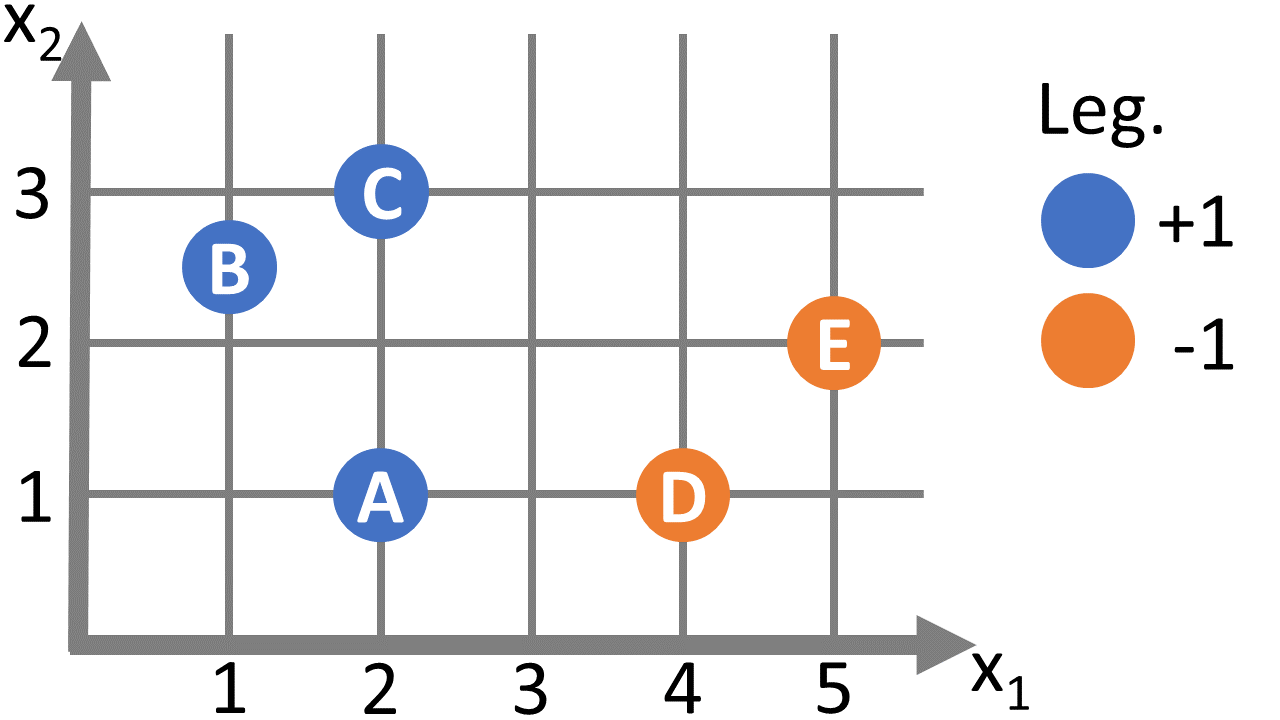
\includegraphics[width=\textwidth]{PowerPoint/Folie9.png}
                        % \caption{Beispiel eines Training-Sets}
                        \label{Bsp_1:fig_1}
                    }
                \end{figure}
            }\only<2->{
                \begin{figure}[h]
                    \centering{
                        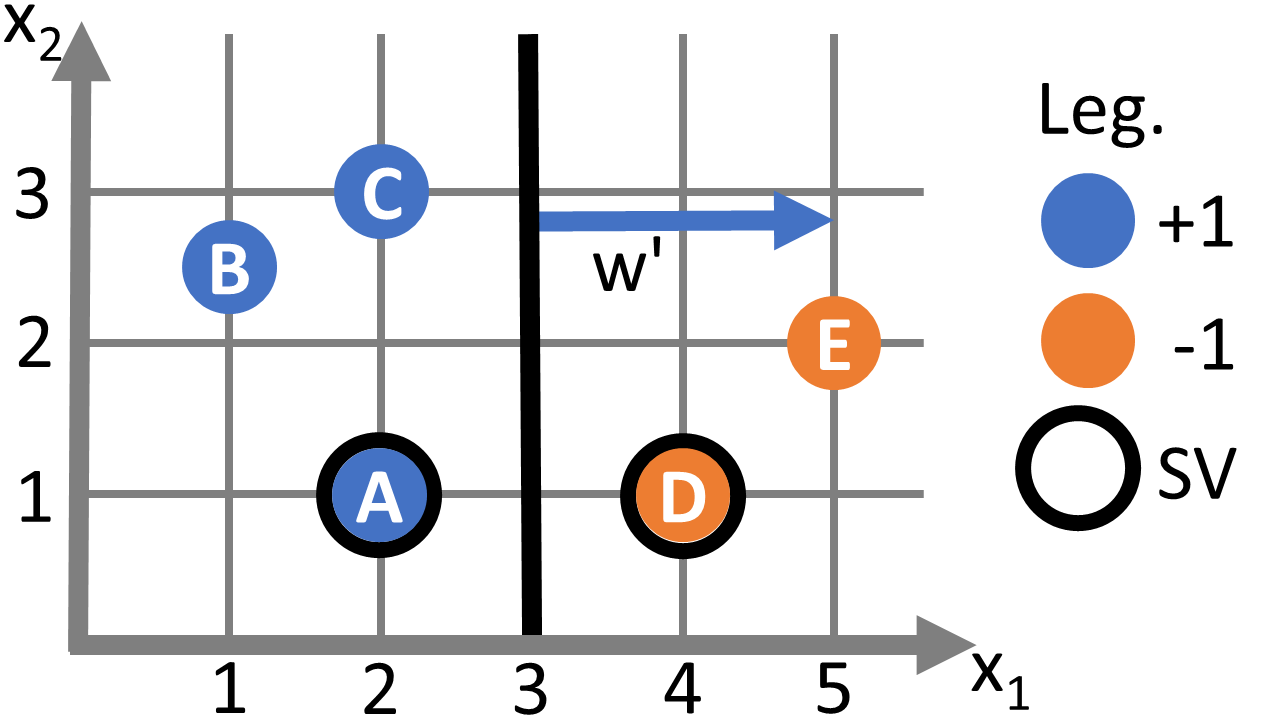
\includegraphics[width=\textwidth]{PowerPoint/Folie10.png}
                        % \caption{Beispiel eines Training-Sets}
                        \label{Bsp_1:fig_2}
                    }
                \end{figure}
            }
        \end{minipage}
        \hfill
        \begin{minipage}{0.4\textwidth}
            \begin{itemize}
                \item<1-> Hyperebene: $ H = \boldsymbol{w} \cdot \boldsymbol{x} + b = 0 $
                \item<1-> Gutter constraint: $ \boldsymbol{w} \cdot \boldsymbol{x}_i + b = y_i, \quad \forall \text{ s. v. } \in \boldsymbol{x} $
            \end{itemize} 
        \end{minipage}
    \end{figure}

    \begin{itemize}
        \item <2-> Graphische Bestimmung der Hyperebenenparameter:
            \begin{align*}
                x &= 3 \\
                \boldsymbol{w} &= \left( \begin{matrix}
                    2 \\
                    0 \\
                \end{matrix} \right) \\
                \left( \begin{matrix}
                    2 & 0 \\
                \end{matrix} \right) \cdot \left( \begin{matrix}
                    3 \\
                    0 \\
                \end{matrix} \right) + b = 0 &\Rightarrow b = -6 \\
            \end{align*}
    \end{itemize}
\end{frame}

%%%%%%%%%%%%%%%%%%%%%%%%%%%%%%%%%%%%%%%%%%%%%%%%%%%%%%%%%%%%%%%%%%%%%%%%%%%%%%%%
% Folie 7: Beispiel II
%%%%%%%%%%%%%%%%%%%%%%%%%%%%%%%%%%%%%%%%%%%%%%%%%%%%%%%%%%%%%%%%%%%%%%%%%%%%%%%%
\begin{frame}
    \frametitle{Beispiel II}

    \begin{figure}[h]
        \begin{minipage}{0.4\textwidth} 
            \only<1>{
                \begin{figure}[h]
                    \centering{
                        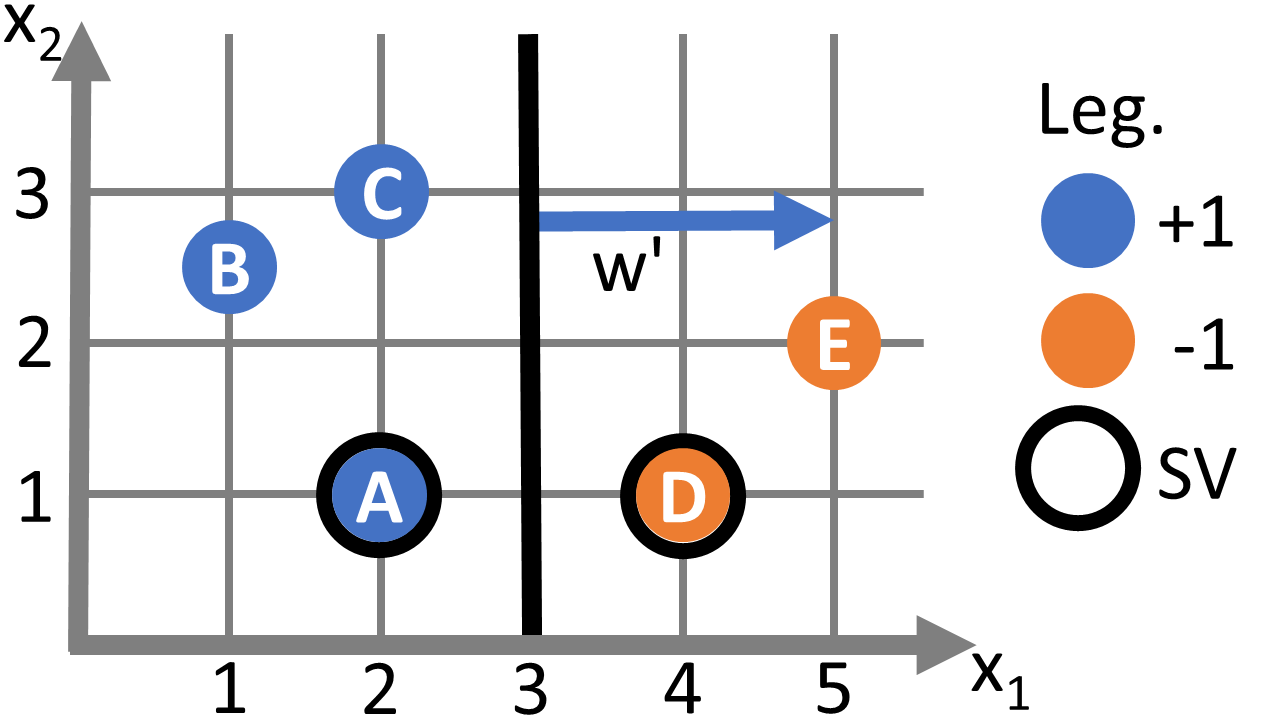
\includegraphics[width=\textwidth]{PowerPoint/Folie10.png}
                        % \caption{Beispiel eines Training-Sets}
                        \label{Bsp_1:fig_2}
                    }
                \end{figure}
            }\only<2->{
                \begin{figure}[h]
                    \centering{
                        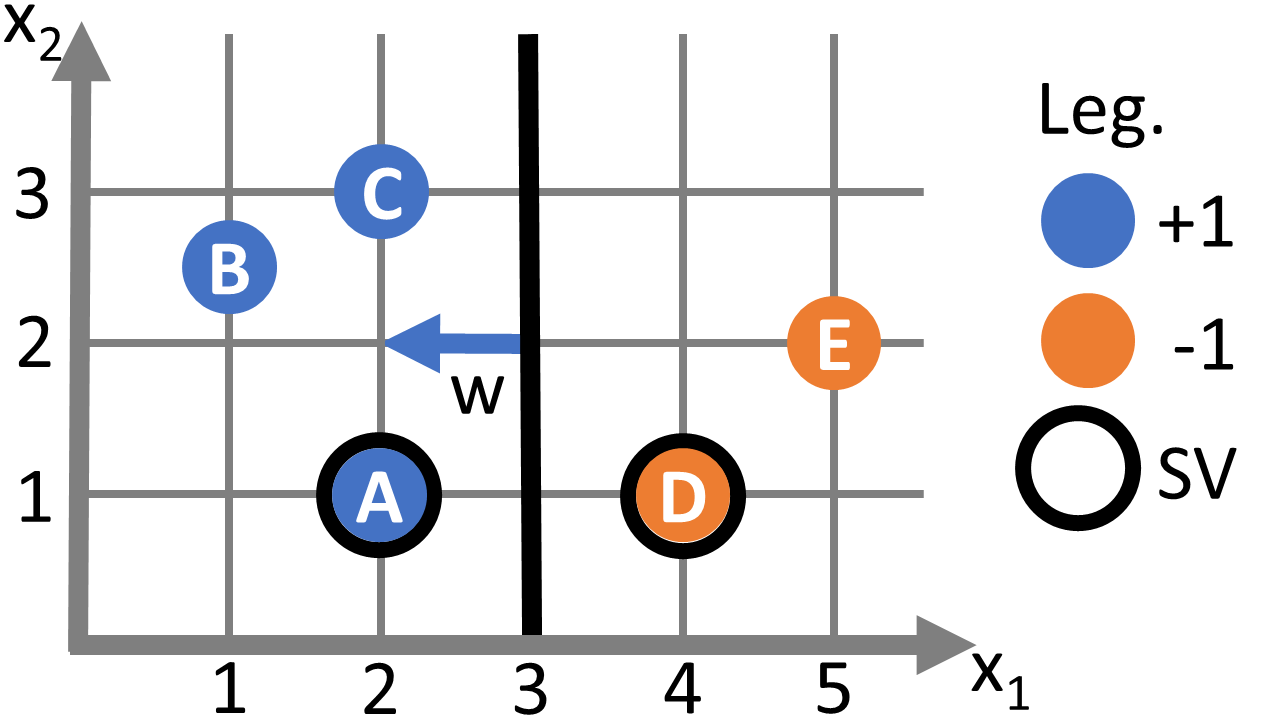
\includegraphics[width=\textwidth]{PowerPoint/Folie11.png}
                        % \caption{Beispiel eines Training-Sets}
                        \label{Bsp_1:fig_2}
                    }
                \end{figure}
            }
        \end{minipage}
        \hfill
        \begin{minipage}{0.4\textwidth}
            \begin{itemize}
                \item<1-> Hyperebene: $ H = \boldsymbol{w} \cdot \boldsymbol{x} + b = 0 $
                \item<1-> Gutter constraint: $ \boldsymbol{w} \cdot \boldsymbol{x}_i + b = y_i, \quad \forall \text{ s. v. } \in \boldsymbol{x} $
            \end{itemize} 
        \end{minipage}
    \end{figure}

    \begin{itemize}
        \item<1-> Berücksichtigen der Gutter constraint am Bsp. von Punkt $A$:
            \begin{align*}
                c \left( \left( \begin{matrix}
                    2 & 0 \\
                \end{matrix} \right) \cdot \left( \begin{matrix}
                    2 \\
                    1 \\
                \end{matrix} \right) - 6 \overset{!}{=} +1 \right) &\Rightarrow c = -0.5 \\
            \end{align*}
        \item<2-> Somit gilt für die kanonische Hyperebene:
            \begin{align*}
                \boldsymbol{w} &= \left( \begin{matrix}
                    -1 \\
                    0 \\
                \end{matrix} \right) \\
                b &= 3 \\ 
            \end{align*}
        \item<3-> Kontrolle mit Punkt $D$:
            \begin{align*}
                \left( \begin{matrix}
                    -1 & 0 \\
                \end{matrix} \right) \cdot \left( \begin{matrix}
                    4 \\
                    1 \\
                \end{matrix} \right) + 3 = -1
            \end{align*}
    \end{itemize}
\end{frame}

%%%%%%%%%%%%%%%%%%%%%%%%%%%%%%%%%%%%%%%%%%%%%%%%%%%%%%%%%%%%%%%%%%%%%%%%%%%%%%%%
% Folie 8: Beispiel III
%%%%%%%%%%%%%%%%%%%%%%%%%%%%%%%%%%%%%%%%%%%%%%%%%%%%%%%%%%%%%%%%%%%%%%%%%%%%%%%%
\begin{frame}
    \frametitle{Beispiel III}

    \begin{figure}[h]
        \begin{minipage}{0.4\textwidth} 
            \only<1->{
                \begin{figure}[h]
                    \centering{
                        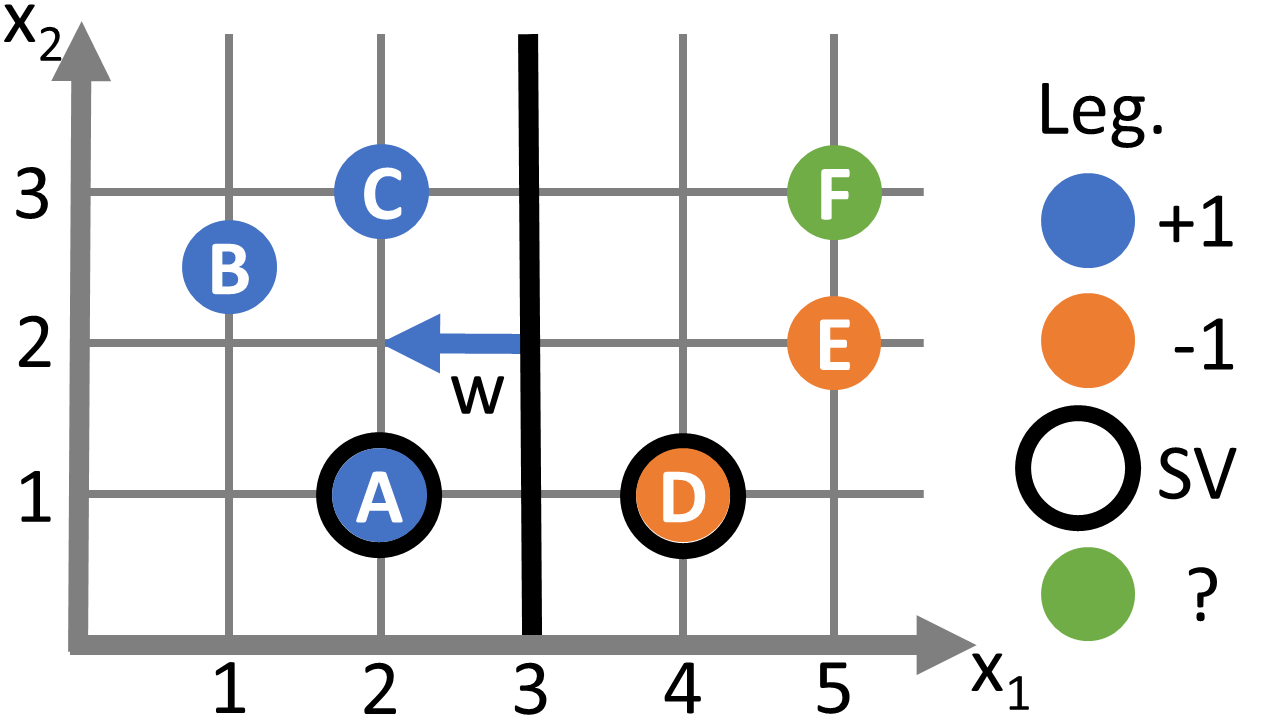
\includegraphics[width=\textwidth]{PowerPoint/Folie12.png}
                        % \caption{Beispiel eines Training-Sets}
                        \label{Bsp_1:fig_2}
                    }
                \end{figure}
            }
        \end{minipage}
        \hfill
        \begin{minipage}{0.4\textwidth}
            \begin{itemize}
                \item<1-> Klassifizierung:
                    \begin{equation*}
                        h(x_i) = \begin{cases}
                            +1 & \text{if } \boldsymbol{w} \cdot \boldsymbol{x}_i + b \geq 0 \\
                            -1 & \text{if } \boldsymbol{w} \cdot \boldsymbol{x}_i + b \leq 0 \\
                        \end{cases}
                    \end{equation*}
                \item<1-> Parameter der kanonischen Hyperebene
                    \begin{align*}
                        \boldsymbol{w} &= \left( \begin{matrix}
                            -1 \\
                            0 \\
                        \end{matrix} \right) \\
                        b &= 3 \\ 
                    \end{align*}
            \end{itemize} 
        \end{minipage}
    \end{figure}

    \begin{itemize}
        \item<1-> Klassifizierung von Punkt $F$:
            \begin{align*}
                \left( \begin{matrix}
                    -1 & 0 \\
                \end{matrix} \right) \cdot \left( \begin{matrix}
                    5 \\
                    3 \\
                \end{matrix} \right) + 3 = -2
            \end{align*}
        \item<1-> Punkt F gehört also zur Klasse $-1$.
    \end{itemize}
\end{frame}

%%%%%%%%%%%%%%%%%%%%%%%%%%%%%%%%%%%%%%%%%%%%%%%%%%%%%%%%%%%%%%%%%%%%%%%%%%%%%%%%
% Folie 9: Minimierungsproblem
%%%%%%%%%%%%%%%%%%%%%%%%%%%%%%%%%%%%%%%%%%%%%%%%%%%%%%%%%%%%%%%%%%%%%%%%%%%%%%%%
\begin{frame}
    \frametitle{Minimierungsproblem}

    \begin{figure}[h]
        \begin{minipage}{0.4\textwidth} 
            \only<1->{
                \begin{figure}[h]
                    \centering{
                        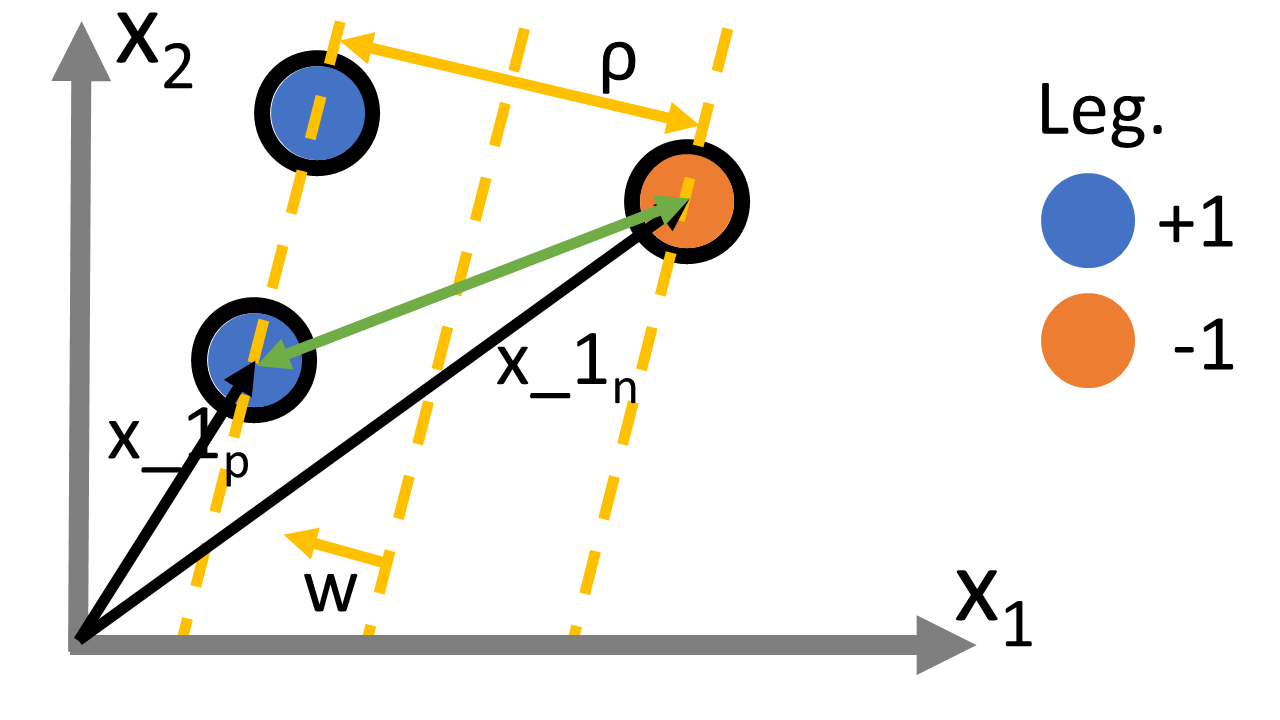
\includegraphics[width=\textwidth]{PowerPoint/Folie8.png}
                        % \caption{Beispiel eines Training-Sets}
                        \label{Min_Prob:fig_1}
                    }
                \end{figure}
            }
        \end{minipage}
        \hfill
        \begin{minipage}{0.4\textwidth}
            \begin{itemize}
                \item Projektionseigenschaft des Skalarprodukts
                \item Breite des margin $\rho$:
                    \begin{equation*}
                        \rho = (\boldsymbol{x_p} - \boldsymbol{x_n}) \cdot \frac{\boldsymbol{w}}{\Vert \boldsymbol{w} \Vert}
                    \end{equation*}
                \item Gutter constraint: 
                    \begin{equation*}
                        y_i ( \boldsymbol{w} \cdot \boldsymbol{x}_i + b ) = 1 \quad \forall \text{ support vectors } \in \boldsymbol{x}
                    \end{equation*}
            \end{itemize} 
        \end{minipage}

        \begin{itemize}
            \item $ \rho = \frac{2}{\Vert \boldsymbol{w} \Vert} $
            \item Ziel einer SVM: Maximiere den margin
                \begin{align*}
                    & \max \frac{2}{\Vert \boldsymbol{w} \Vert} \Leftrightarrow \min \Vert \boldsymbol{w} \Vert \Leftrightarrow \min \frac{1}{2} \Vert \boldsymbol{w} \Vert^2 \\
                    & \text{u.d.N. } y_i ( \boldsymbol{w} \cdot \boldsymbol{x}_i + b ) - 1 \geq 0 \\
                \end{align*}
        \end{itemize}
    \end{figure}
\end{frame}

%%%%%%%%%%%%%%%%%%%%%%%%%%%%%%%%%%%%%%%%%%%%%%%%%%%%%%%%%%%%%%%%%%%%%%%%%%%%%%%%
% Folie 10: Lagrange multipliers
%%%%%%%%%%%%%%%%%%%%%%%%%%%%%%%%%%%%%%%%%%%%%%%%%%%%%%%%%%%%%%%%%%%%%%%%%%%%%%%%
\begin{frame}
    \frametitle{Lagrange multipliers}

    \begin{itemize}
        \item Langrange multipliers:
            \begin{align*}
                L = \frac{1}{2} \Vert \boldsymbol{w} \Vert^2 - \sum \alpha_i \left[ y_i ( \boldsymbol{w} \cdot \boldsymbol{x}_i + b) - 1 \right] \\
            \end{align*}
        \item Suche nach den Extremum
            \begin{align*}
                \frac{\partial L}{\partial \boldsymbol{w}} = \boldsymbol{w} - \sum \alpha_i y_i \boldsymbol{x}_i = 0 &\Rightarrow \boldsymbol{w} = \sum_i \alpha_i y_i \boldsymbol{x}_i \\
                \frac{\partial L}{\partial b} = -\sum \alpha_i y_i = 0 &\Rightarrow \sum_i \alpha_i y_i = 0 \\
            \end{align*}
        \item $\boldsymbol{w}$ in $L$ eingesetzt:
            \begin{align*}
                L &= \frac{1}{2} (\sum_i \alpha_i y_i \boldsymbol{x}_i) \cdot (\sum_j \alpha_j y_j \boldsymbol{x}_j) - (\sum_i \alpha_i y_i \boldsymbol{x}_i) \cdot (\sum_j \alpha_j y_j \boldsymbol{x}_j) - \sum_i \alpha_i y_i b + \sum_i \alpha_i \\
                L &= \sum_i \alpha_i - \frac{1}{2} \sum_i \sum_j \alpha_i \alpha_j y_i y_j \boldsymbol{x}_i \cdot \boldsymbol{x}_j
            \end{align*}
        \item Ziel: $ \max L$
        \item Entscheidungsfunktion:
            \begin{align*}
                h(\boldsymbol{u}) = \sum_i \alpha_i y_i \boldsymbol{x}_i \cdot \boldsymbol{u} + b \begin{cases}
                    \geq 0 & \Rightarrow y_u = +1 \\
                    \leq 0 & \Rightarrow y_u = -1 \\
                \end{cases}
            \end{align*}
    \end{itemize}
\end{frame}

%%%%%%%%%%%%%%%%%%%%%%%%%%%%%%%%%%%%%%%%%%%%%%%%%%%%%%%%%%%%%%%%%%%%%%%%%%%%%%%%
% Folie 11: supportiveness values
%%%%%%%%%%%%%%%%%%%%%%%%%%%%%%%%%%%%%%%%%%%%%%%%%%%%%%%%%%%%%%%%%%%%%%%%%%%%%%%%
\begin{frame}
    \frametitle{Supportiveness values $\alpha$}

    \begin{itemize}
        \item Eigenschaften:
            \begin{align*}
                & \boldsymbol{\alpha} \geq 0 \\
                & \alpha_i \begin{cases}
                    > 0 & \text{ wenn } x_i \text{ ein support vector ist} \\
                    = 0 & \text{ sonst} \\
                \end{cases} \\
            \end{align*}
        \item $ \sum\limits_{\substack{ \text{s.v.} \\ i}} \alpha_i y_i  = 0 \Leftrightarrow \sum\limits_{\substack{ \text{pos. s.v.} \\ p}} \alpha_p  = \sum\limits_{\substack{ \text{neg. s.v.} \\ n}} \alpha_n $
        \item $ \sum\limits_i \alpha_i y_i \boldsymbol{x}_i = \boldsymbol{w} \Leftrightarrow \boldsymbol{w} = \sum\limits_p \alpha_p \boldsymbol{x}_p - \sum\limits_n \alpha_n \boldsymbol{x}_n $
    \end{itemize}

    \vspace{3mm}

    \only<2>{
        \begin{figure}[h]
            \begin{minipage}{0.4\textwidth} 
                \begin{figure}[h]
                    \centering{
                        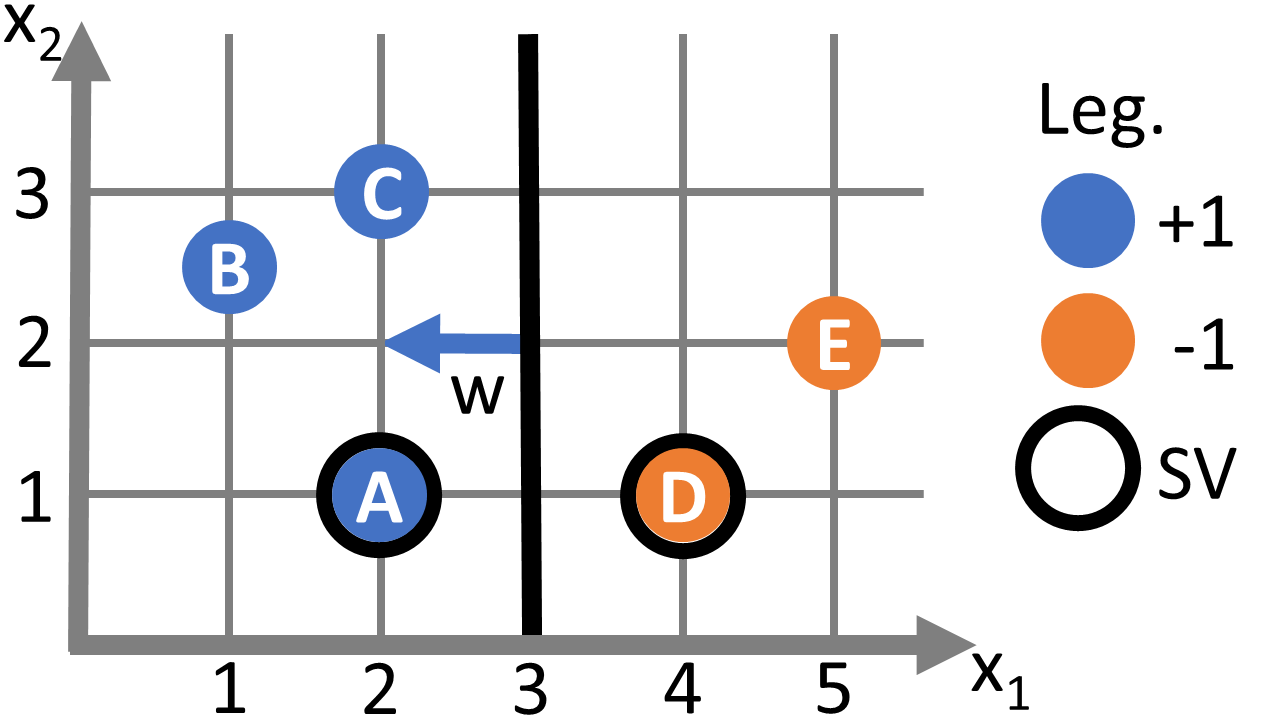
\includegraphics[width=\textwidth]{PowerPoint/Folie11.png}
                        % \caption{Beispiel eines Training-Sets}
                        \label{Bsp_1:fig_2}
                    }
                \end{figure}
            \end{minipage}
            \hfill
            \begin{minipage}{0.4\textwidth}
                \begin{itemize}
                    \item Berechnung von $\alpha_A$ und $\alpha_D$ ergibt:
                        \begin{align*}
                            \alpha_A &= 0.5 \\
                            \alpha_D &= 0.5
                        \end{align*}
                \end{itemize}

                \begin{itemize}
                    \item Berechnung von $\alpha_C$ ergibt:
                        \begin{align*}
                            \alpha_C = 0
                        \end{align*}
                \end{itemize}
            \end{minipage}
        \end{figure}
    }
\end{frame}

%%%%%%%%%%%%%%%%%%%%%%%%%%%%%%%%%%%%%%%%%%%%%%%%%%%%%%%%%%%%%%%%%%%%%%%%%%%%%%%%
% Folie 12: Zusammenfassung
%%%%%%%%%%%%%%%%%%%%%%%%%%%%%%%%%%%%%%%%%%%%%%%%%%%%%%%%%%%%%%%%%%%%%%%%%%%%%%%%
\begin{frame}
    \frametitle{Zusammenfassung}

    \begin{itemize}
        \item Kanonische Hyperebene:
            \begin{align*}
                \boldsymbol{w} \cdot \boldsymbol{x} + b = 0
            \end{align*}
        \item Gesucht: Parameter $\boldsymbol{w}$ und $b$
        \item Supportive values $\alpha$:
            \begin{align*}
                \boldsymbol{w} = \sum_i \alpha_i y_i \boldsymbol{x}_i \\
                \sum_i \alpha_i y_i = 0 \\
            \end{align*}
        \item Entscheidungsfunktion $H$:
            \begin{align*}
                h(\boldsymbol{u}) = \sum_j \alpha_j y_j \boldsymbol{x}_j \cdot \boldsymbol{u} + b \begin{cases}
                    \geq 0 & \Rightarrow y_u = +1 \\
                    \leq 0 & \Rightarrow y_u = -1 \\
                \end{cases}
            \end{align*}
        \item Supportvektoren
            \begin{align*}
                & y_i (\sum_j \alpha_j y_j \boldsymbol{x}_j \cdot \boldsymbol{x}_i + b) = 1 \quad \forall \text{ s.v. } \boldsymbol{x}_i \in \boldsymbol{x} \\
                & \alpha_i \begin{cases}
                    > 0 & \text{ wenn } x_i \text{ ein support vector ist} \\
                    = 0 & \text{ sonst} \\
                \end{cases} \\
            \end{align*}
    \end{itemize}
\end{frame}

  \section{Einführung}
	\begin{frame}
		\frametitle{Einführung: Linear separierbare Daten}
			\begin{figure}
					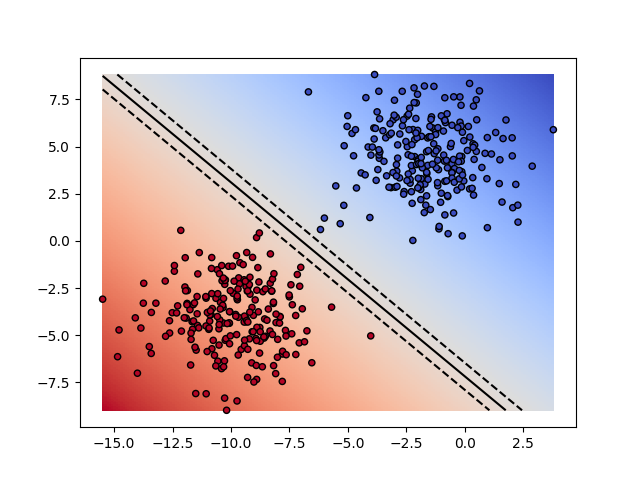
\includegraphics[width=\textwidth]{img/linearsvm.png}
			\end{figure}
	\end{frame}
	
	\begin{frame}
		\frametitle{Einführung: Linear nicht separierbare Daten 1}
			\begin{figure}
					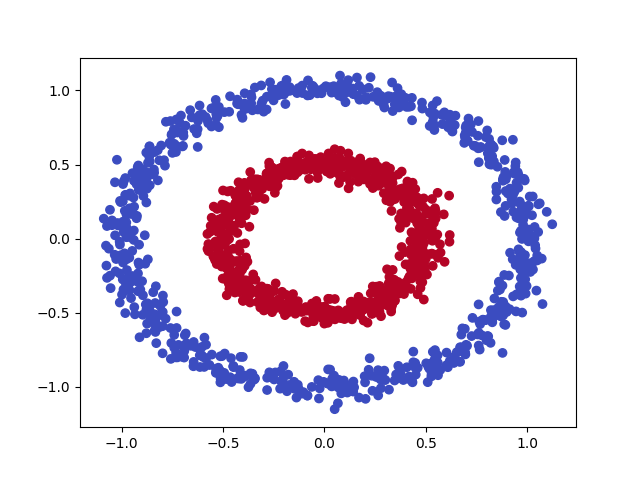
\includegraphics[width=\textwidth]{img/nonlinearsvm.png}
			\end{figure}
	\end{frame}
	
	\begin{frame}
		\frametitle{Einführung: Linear nicht separierbare Daten 2}
			\begin{figure}
					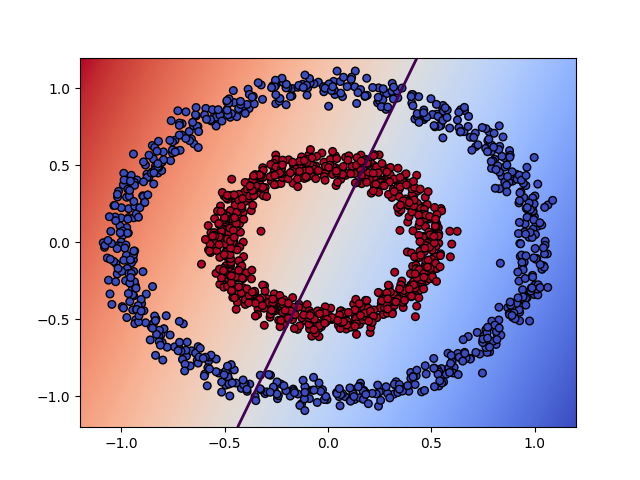
\includegraphics[width=\textwidth]{img/nonlinearsvmwbl.png}
			\end{figure}
	\end{frame}
	
	\begin{frame}
		\frametitle{Ansatz: Einführung}
			\begin{columns}
				\begin{column}{.4\textwidth}
					\begin{figure}
						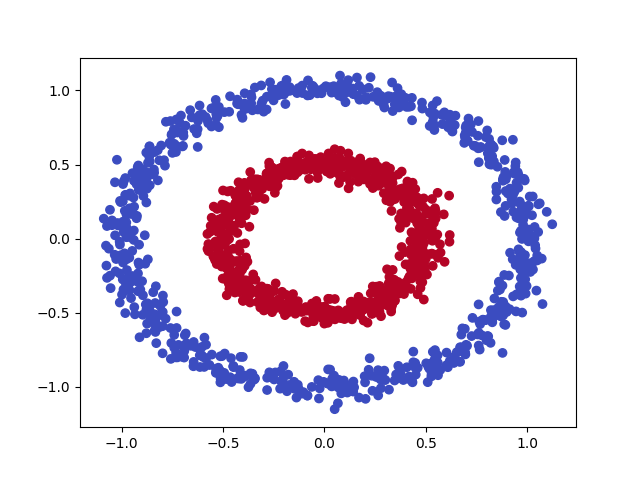
\includegraphics[width=1\textwidth]{img/nonlinearsvm.png}
					\end{figure}
					\begin{align*}
						\phi(\boldsymbol{x}) &=  \begin{bmatrix}
										x_{1} \\
										x_{2} \\
										x_{1}^{\,2} + x_{2}^{\,2}
									\end{bmatrix}
					\end{align*}
				\end{column}
				\begin{column}{.6\textwidth}
				\end{column}
			\end{columns}
	\end{frame}
	\begin{frame}
	\frametitle{Ansatz: Einführung}
		\begin{columns}
			\begin{column}{.4\textwidth}
				\begin{figure}
					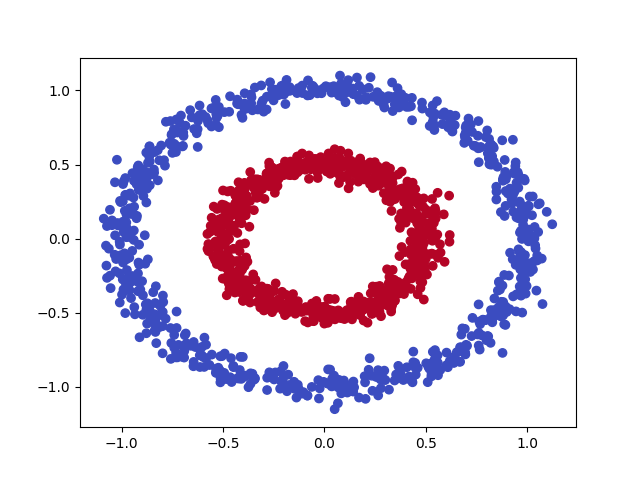
\includegraphics[width=1\textwidth]{img/nonlinearsvm.png}
				\end{figure}
				\begin{align*}
					\phi(\boldsymbol{x}) &=  \begin{bmatrix}
									x_{1} \\
									x_{2} \\
									x_{1}^{\,2} + x_{2}^{\,2}
								\end{bmatrix}
				\end{align*}
			\end{column}
			\begin{column}{.6\textwidth}
				\begin{figure}
					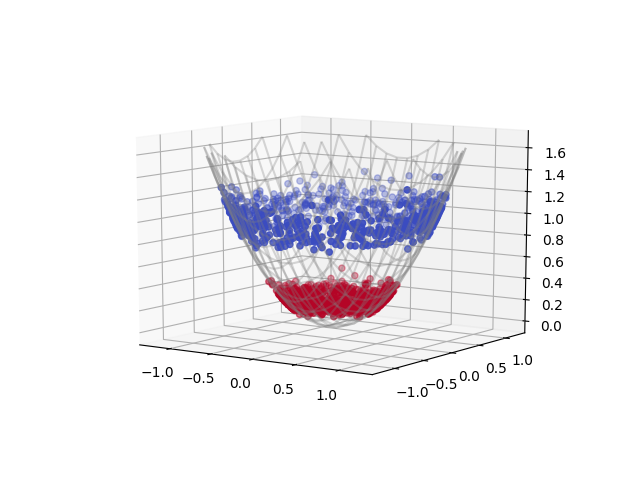
\includegraphics[width=1\textwidth]{img/nonlinearsvm3d.png}
				\end{figure}
				\vspace{45pt}
			\end{column}
		\end{columns}
	\end{frame}
	
	\begin{frame}
		\frametitle{Ansatz: Abbildfunktion $\phi(x)$}
			\begin{columns}
				\begin{column}{.6\textwidth}
					\begin{figure}
							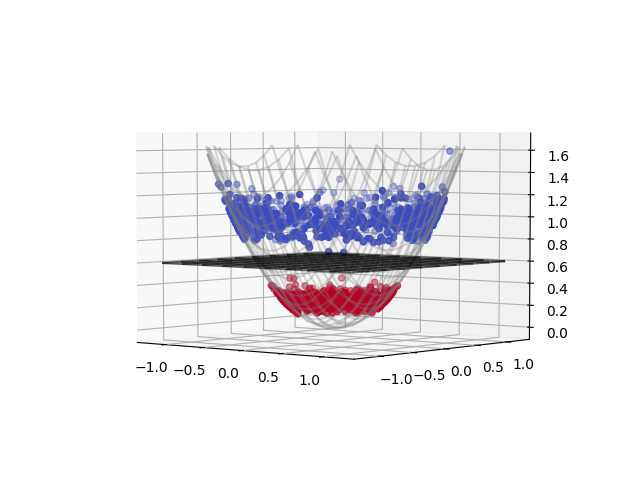
\includegraphics[width=1\textwidth]{img/nonlinearsvm3dwb.png}
					\end{figure}
				\end{column}
				\begin{column}{.4\textwidth}
					\begin{figure}
							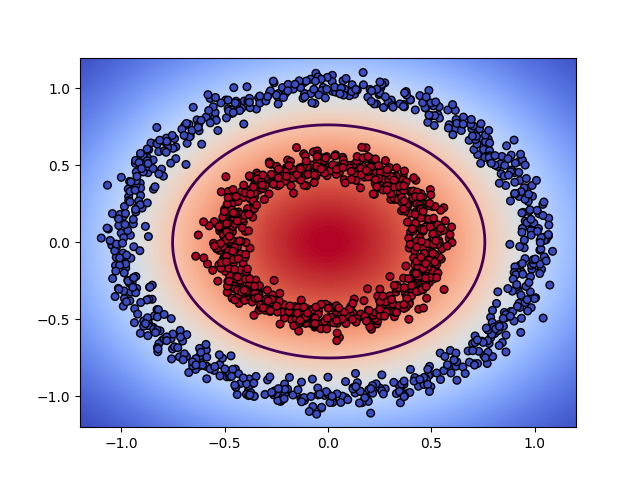
\includegraphics[width=1\textwidth]{img/nonlinearsvmwb.png}
					\end{figure}
				\end{column}
			\end{columns}
	\end{frame}
	
	\begin{frame}
		\frametitle{Veränderung der Funktionen}
			\begin{equation*}
				L = \sum_i \alpha_i - \frac{1}{2} \sum_i \sum_j \alpha_i \alpha_j y_i y_j \boldsymbol{x}_i^{T} \boldsymbol{x}_j
			\end{equation*}
			\onslide<2->{
				\begin{equation*}
					L = \sum_i \alpha_i - \frac{1}{2} \sum_i \sum_j \alpha_i \alpha_j y_i y_j \textcolor{red}{\phi(}\boldsymbol{x}_i\textcolor{red}{)}^{T} \textcolor{red}{\phi(}\boldsymbol{x}_j\textcolor{red}{)}
				\end{equation*}
			}
			\begin{equation*}
				h(\boldsymbol{x}) = \sum_i \alpha_i y_i \boldsymbol{x}_i^{T} \boldsymbol{x} + b
			\end{equation*}
			\onslide<2->{
				\begin{equation*}
					h(\boldsymbol{x}) = \sum_i \alpha_i y_i \textcolor{red}{\phi(}\boldsymbol{x}_i\textcolor{red}{)}^{T} \textcolor{red}{\phi(}\boldsymbol{x}\textcolor{red}{)} + b
				\end{equation*}
			}
	\end{frame}

\section{Mathematik}
	\begin{frame}
		\frametitle{Definition: $\phi$}
			Abbildfunktion
			\begin{align*}
				\phi: \mathbb{R}^{n} & \to \mathbb{R}^{m} \\
				\boldsymbol{x} & \mapsto \boldsymbol{f}
			\end{align*}
			\pause
			Probleme:
			\begin{itemize}
				\item $m > n$ höherer Rechenaufwand \\
					Ab einer bestimmten Größe kann damit nicht mehr gerechnet werden
				\item Obergrenze für $m$
				\item $\phi$ nur für Skalarprodukt benötigt
			\end{itemize}
	\end{frame}
	
	\begin{frame}
		\frametitle{Beispiel Kernel}
			\begin{equation*}
				\phi(\boldsymbol{x}) = (1 \ \sqrt{2}x_{1} \ \sqrt{2}x_{2} \ \dots \ x_{1}^{2} \ x_{2}^{2} \ \dots \ \sqrt{2}x_{1}x_{2} \ \sqrt{2}x_{1}x_{3} \ \dots)
			\end{equation*}
			\pause
			\begin{align*}
				\phi(\boldsymbol{v})^{T}\phi(\boldsymbol{w}) &= \sum_{j} 2v_{j}w_{j} + \sum_{j} v_{j}^{2} w_{j}^{2} + \sum_{j} \sum_{k > j} 2 v_{j} v_{k} w_{j} w_{k} + \dots \\
						&= (1+\sum_{j} v_{j} w_{j})^{2} \\
						&= (1+\boldsymbol{v}^{T} \boldsymbol{w})^{2} \\
						&= K(\boldsymbol{v}, \boldsymbol{w})
			\end{align*}
	\end{frame}
	
	\begin{frame}
		\frametitle{Einführung von Kerneln}
			\begin{align*}
				K&(\boldsymbol{v}, \boldsymbol{w}) = \phi(\boldsymbol{v})^{T} \phi(\boldsymbol{w})\\
				K&: \mathbb{R}^n \times \mathbb{R}^n \rightarrow \mathbb{R}
			\end{align*}
			\pause
			\begin{equation*}
				L = \sum_i \alpha_i - \frac{1}{2} \sum_i \sum_j \alpha_i \alpha_j y_i y_j \textcolor{red}{K(}\boldsymbol{x}_i\textcolor{red}{,} \boldsymbol{x}_j\textcolor{red}{)}
			\end{equation*}
			\begin{equation*}
				h(\boldsymbol{x}) = \sum_i \alpha_i y_i \textcolor{red}{K(}\boldsymbol{x}_i\textcolor{red}{,} \boldsymbol{x}\textcolor{red}{)} + b
			\end{equation*}
	\end{frame}
	
	\begin{frame}
		\frametitle{Mercer's Theorem: 1}
			$\{ \boldsymbol{x}^{(1)}, \dots, \boldsymbol{x}^{(m)} \}$ \\
			$\mathcal{K}_{i,j} = K(\boldsymbol{x}^{(i)}, \boldsymbol{x}^{(j)})$ \\\
			\pause
			
			\begin{align*}
				\mathcal{K}_{i,j} &= K(\boldsymbol{x}^{(i)}, \boldsymbol{x}^{(j)}) \\
								  &= \phi(\boldsymbol{x}^{(i)})^{T} \phi(\boldsymbol{x}^{(j)}) \\
								  &= \phi(\boldsymbol{x}^{(j)})^{T} \phi(\boldsymbol{x}^{(i)}) \\
								  &= K(\boldsymbol{x}^{(j)}, \boldsymbol{x}^{(i)}) \\
								  &= \mathcal{K}_{j,i}
			\end{align*}
	\end{frame}
	
	\begin{frame}
		\frametitle{Mercer's Theorem: 2}
			$\{ \boldsymbol{x}^{(1)}, \dots, \boldsymbol{x}^{(m)} \}$ \\
			$\mathcal{K}_{i,j} = K(\boldsymbol{x}^{(i)}, \boldsymbol{x}^{(j)})$ \\\
			
			Wähle $\boldsymbol{z}$ beliebig:
			\begin{align*}
				\boldsymbol{z}^{T} \mathcal{K} \boldsymbol{z} &= \sum_{i} \sum_{j} \boldsymbol{z}_{i} \mathcal{K}_{i,j} \boldsymbol{z}_{j} \\
															  &= \sum_{i} \sum_{j} \boldsymbol{z}_{i} \phi(\boldsymbol{x}^{(i)})^{T} \phi(\boldsymbol{x}^{(j)}) \boldsymbol{z}_{j} \\
															  &= \sum_{i} \sum_{j} \boldsymbol{z}_{i} \sum_{k} \phi_{k}(\boldsymbol{x}^{(i)}) \phi_{k}(\boldsymbol{x}^{(j)}) \boldsymbol{z}_{j} \\
															  &= \sum_{k} \sum_{i} \sum_{j} \boldsymbol{z}_{i} \phi_{k}(\boldsymbol{x}^{(i)}) \phi_{k}(\boldsymbol{x}^{(j)}) \boldsymbol{z}_{j} \\
															  &= \sum_{k} \left( \sum_{i} \boldsymbol{z}_{i} \phi_{k}(\boldsymbol{x}^{(i)}) \right)^{2} \\
															  &\ge 0 \\
			\end{align*}
	\end{frame}
	
	% \begin{frame}
	% 	\frametitle{Kernel Operationen: Addition}
	% 		Addition \\
	% 		\begin{align*}
	% 			(K_{1} + K_{2})(\boldsymbol{v}, \boldsymbol{w}) &= K_{1}(\boldsymbol{v}, \boldsymbol{w}) + K_{2}(\boldsymbol{v}, \boldsymbol{w}) \\
	% 			&= \phi_{1}(\boldsymbol{v})^{T}\phi_{1}(\boldsymbol{w}) + \phi_{2}(\boldsymbol{v})^{T}\phi_{2}(\boldsymbol{w}) \\
	% 			&= (\phi_{1}(\boldsymbol{v}), \phi_{2}(\boldsymbol{v})) \left( \begin{matrix}
	% 													  	\phi_{1}(\boldsymbol{w}) \\
	% 													  	\phi_{2}(\boldsymbol{w})
	% 													  \end{matrix} \right)
	% 		\end{align*}
	% \end{frame}
	% \begin{frame}
	% 	\frametitle{Kernel Operationen: Multiplikation}
	% 		Multiplikation \\
	% 		\begin{align*}
	% 			(K_{1} \times K_{2})(\boldsymbol{v}, \boldsymbol{w}) &= K_{1}(\boldsymbol{v}, \boldsymbol{w}) K_{2}(\boldsymbol{v}, \boldsymbol{w}) \\
	% 			&= \sum_{i=1}^{n} \phi_{1i}(\boldsymbol{v})\phi_{1i}(\boldsymbol{w}) \sum_{j=1}^{m} \phi_{2j}(\boldsymbol{v})\phi_{2j}(\boldsymbol{w}) \\
	% 			&= \sum_{i=1}^{n} \sum_{j=1}^{m} (\phi_{1i}(\boldsymbol{v})\phi_{2j}(\boldsymbol{v}))(\phi_{1i}(\boldsymbol{w})\phi_{2j}(\boldsymbol{w})) \\
	% 			&= \sum_{k=1}^{nm} \phi_{12k}(\boldsymbol{v})\phi_{12k}(\boldsymbol{w}) = \phi_{12}(\boldsymbol{v})^{T}\phi_{12k}(\boldsymbol{w})
	% 		\end{align*}
	% 		Mit $\phi_{12}(\boldsymbol{x}) = \phi_{1}(\boldsymbol{x}) \times \phi_{2}(\boldsymbol{x})$ dem kartesischen Produkt
	% \end{frame}
	
	\begin{frame}
		\frametitle{Verschiedene Kernel in der Praxis}
			\begin{itemize}
				\item Linearer Kernel \\
				\item Polynomiell \\
				\item Gauß'schen Kernel \\
				\item Esotherische Kernel \\
			\end{itemize}
	\end{frame}

	\begin{frame}
		\frametitle{Verschiedene Kernel in der Praxis: Linear}
			\vspace{10pt}
			$K(\boldsymbol{v}, \boldsymbol{w}) = \boldsymbol{v}^{\, T} \boldsymbol{w}$
			\begin{figure}
				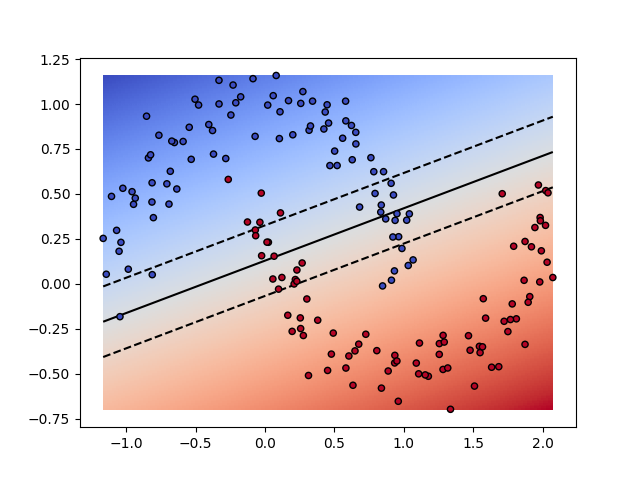
\includegraphics[width=.9\textwidth]{img/kernelLin.png}
			\end{figure}
	\end{frame}
	
	\begin{frame}
		\frametitle{Verschiedene Kernel in der Praxis: Polynomiell}
			\vspace{10pt}
			$K(\boldsymbol{v}, \boldsymbol{w}) = (\boldsymbol{v}^{\, T} \boldsymbol{w} + c)^{d}$
			\begin{figure}
				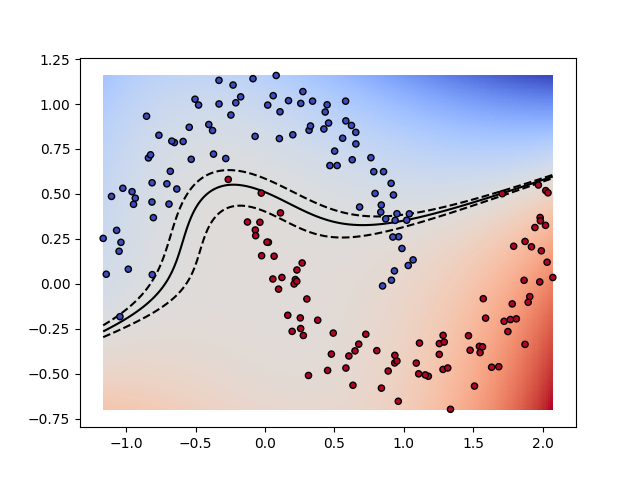
\includegraphics[width=.9\textwidth]{img/kernelPol.png}
			\end{figure}
	\end{frame}
	
	\begin{frame}
		\frametitle{Verschiedene Kernel in der Praxis: Gauß}
			\vspace{10pt}
			$K(\boldsymbol{v}, \boldsymbol{w}) = \exp\left(-\frac{\lvert\lvert\boldsymbol{v} - \boldsymbol{w}\rvert\rvert^{2}}{2\sigma^{2}}\right)$ \\
			
			\begin{figure}
				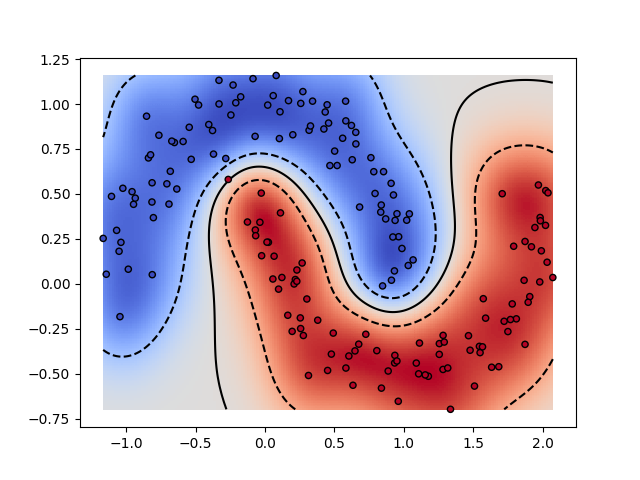
\includegraphics[width=.9\textwidth]{img/kernelGau.png}
			\end{figure}
	\end{frame}
	
	\begin{frame}
		\frametitle{Verschiedene Kernel in der Praxis: Gauß}
			\vspace{10pt}
			$K(\boldsymbol{v}, \boldsymbol{w}) = \exp\left(-\frac{\lvert\lvert\boldsymbol{v} - \boldsymbol{w}\rvert\rvert^{2}}{2\sigma^{2}}\right)$ \\\
			
			\begin{columns}
				\begin{column}{.5\textwidth}
					\begin{figure}
						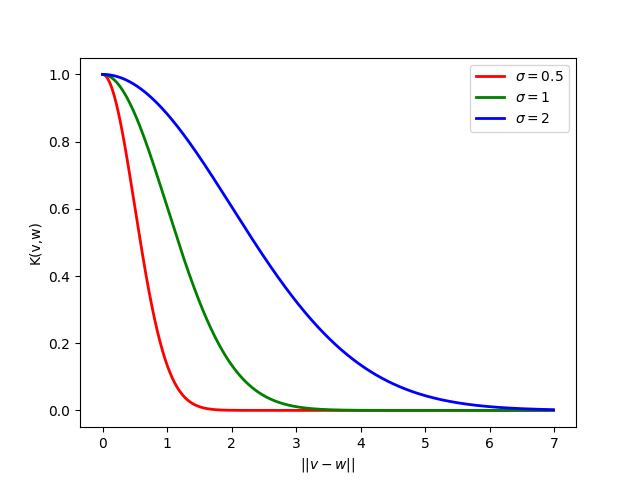
\includegraphics[width=\textwidth]{img/sigmaGau.png}
					\end{figure}
				\end{column}
				\begin{column}{.5\textwidth}
					\begin{figure}
						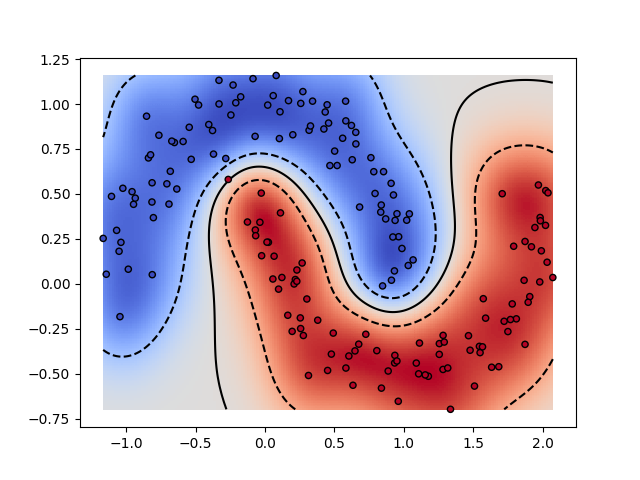
\includegraphics[width=\textwidth]{img/kernelGau.png}
					\end{figure}
				\end{column}
			\end{columns}
	\end{frame}
	
	\begin{frame}
		\frametitle{Verschiedene Kernel in der Praxis: Esotherisch}
			$K: D \times D \rightarrow \mathbb{R}$ \\\
			
			Beispiel: String Kernel \\
			\hspace{31pt} Misst Ähnlichkeit von zwei Strings \\
			\hspace{31pt} Vergleicht verschiedene Aspekte \\
			\hspace{62pt} e.g. Subequenzen, gemeinsame Wörter, Länge, $\dots$
	\end{frame}
	
\section{Zusammenfassung}
	\begin{frame}
		\frametitle{Zusammenfassung}
			\begin{itemize}
				\item SVMs in ihrer Standartform haben Probleme nicht linear trennbare Datensätze zu klassifizieren
				\item Mit $\phi(x)$ Daten in einen Raum abbilden, wo dies möglich ist
				\item Kernel nutzen, um die daraus folgende Berechnung zu vereinfachen
			\end{itemize}
	\end{frame}


\end{document}

